\documentclass[a4paper,11pt]{article}
\usepackage[utf8]{inputenc}
\usepackage{minted}
\usepackage{amsmath}
\usepackage{float}
\usepackage[symbol]{footmisc}
\usepackage{graphicx}
\usepackage[toc,page]{appendix}

\graphicspath{{./figures/}}
\renewcommand{\thefootnote}{\fnsymbol{footnote}}

\title{\textbf{5. Doubly Linked List}}
\author{Kristiāns Vinters}
\date{Fall 2023}

\begin{document}
    \maketitle
    \section*{Introduction}

    I solved the assignment in Go. I used Go because I want to become more familiar with it. Source code and benchmark data is available on GitHub\footnote[1]{https://github.com/Phanty133/id1021/tree/master/4-linkedlist}.

    \section*{Implementation}

    There weren't any particular difficulties implementing doubly linked lists in Go, as Go handles references with C-like pointers. I implemented the structure in a separate \texttt{dllist} package, very similar to the \texttt{llist} package from assignment 4.

    \begin{minted}{go}
type DoublyLinkedListItem[T comparable] struct {
    Head T
    next *DoublyLinkedListItem[T]
    prev *DoublyLinkedListItem[T]
}

type DoublyLinkedList[T comparable] struct {
    first *DoublyLinkedListItem[T]
    last  *DoublyLinkedListItem[T]
}
    \end{minted}

    The \texttt{Remove()} function did not pose any difficulties, as it was just a linear search to find the item then rearranging the pointers and handling the edge cases. I implemented the \texttt{Remove()} function using the \texttt{Unlink} function, as the functionality is almost the same, bar the initial search step.

    \begin{minted}{go}
func (l *DoublyLinkedList[T]) Unlink(item *DoublyLinkedListItem[T]) {
    if item.prev != nil {
        item.prev.next = item.next
    } else {
        l.first = item.next
    }

    if item.next != nil {
        item.next.prev = item.prev
    } else {
        l.last = item.prev
    }
}

func (l *DoublyLinkedList[T]) Remove(value T) {
    if l.first == nil {
        return
    }

    item := l.Find(value)

    if item == nil {
        return
    }

    l.Unlink(item)
}
    \end{minted}

    \section*{Benchmarking}

    I benchmarked the linked list and array by running them 500 times with a $k=1000$ and changing sizes $\left\{10, 100, 1000, 5000, 10000, 15000\right\}$. I generated the $k$ random items as suggested in the assignment description.

    \begin{minted}{go}
a, items := PrepareDLLData(n)

kIdxs := GenRandomInts(k, 0, n)
kItems := make([]*dllist.DoublyLinkedListItem[int], k)

for j := 0; j < k; j++ {
    kItems[j] = items[kIdxs[j]]
}
    \end{minted}

    \begin{figure}[H]
        \centering
        
        \begin{tabular}{c|c|c}
            Size & $t_\text{LL}$, ms & $t_\text{DLL}$, ms \\
            \hline
            \hline
            10 & 0.005 & 0.005 \\
            \hline
            100 & 0.052 & 0.003 \\
            \hline
            1000 & 0.487 & 0.003 \\
            \hline
            5000 & 2.94 & 0.004 \\
            \hline
            10000 & 5.59 & 0.004 \\
            \hline
            15000 & 7.72 & 0.005 \\
        \end{tabular}

        \caption{Median execution times for unlinking then inserting $k$ elements.}
    \end{figure}

    \begin{figure}[H]
        \centering
        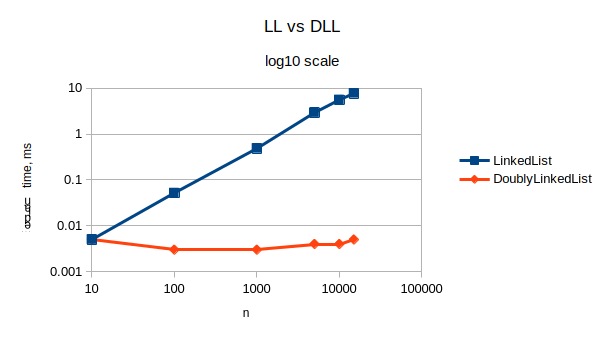
\includegraphics[width=\textwidth]{b3.png}
        \caption{Median execution time}
        \label{fig:b3}
    \end{figure}

    The time complexity for the linked list is $O(n)$, as it has to traverse the entire list to find the item to remove. The time complexity for the doubly linked list is $O(1)$, as it has a reference to the previous item, so it can just unlink the item and insert it at the beginning of the list.
\end{document}